\documentclass[tikz,border=2pt]{standalone}
\usepackage{amsmath,amssymb}
\usepackage{pgfplots}
\pgfplotsset{compat=1.18}
\usetikzlibrary{arrows.meta,decorations.pathreplacing}
\begin{document}
% v = theta_1 + theta_2, theta_2 ~ U[0,1], bidder 1 has theta_1 = 0.6 and wins the first-price
% auction when theta_2 < 0.6: E[v | theta_1] = 1.1 but E[v | theta_1, win] = 0.9; bid 0.6, margin 0.3.
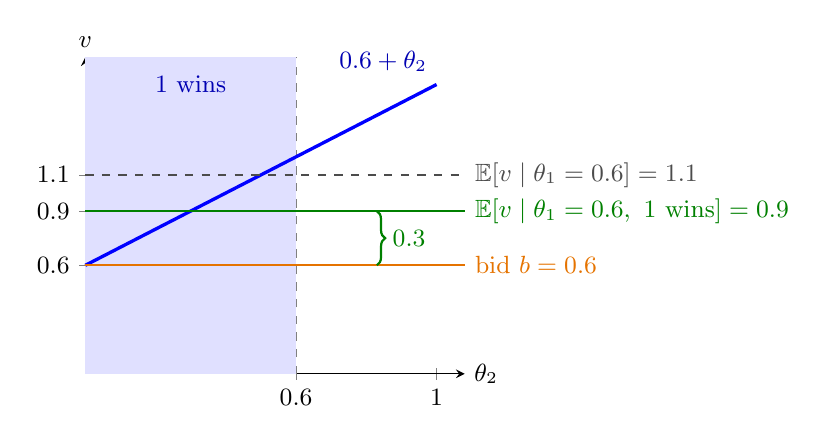
\begin{tikzpicture}[font=\small, >={Latex[length=2mm]}]
  \begin{axis}[
    axis lines=left,
    xmin=0, xmax=1.08, ymin=0, ymax=1.75,
    xtick={0.6,1}, ytick={0.6,0.9,1.1},
    xlabel={$\theta_2$}, ylabel={$v$},
    xlabel style={at={(axis description cs:1,0)}, anchor=west},
    ylabel style={at={(axis description cs:0,1)}, anchor=south, rotate=-90},
    tick label style={font=\small},
    samples=2, clip=false,
    width=6.4cm, height=5.6cm]
    % winning region
    \fill[blue!12] (axis cs:0,0) rectangle (axis cs:0.6,1.75);
    \node[blue!70!black, anchor=south] at (axis cs:0.3,1.5) {1 wins};
    \draw[gray, thin, dashed] (axis cs:0.6,0) -- (axis cs:0.6,1.75);
    % value given theta_1 = 0.6
    \addplot[blue, very thick, domain=0:1] {0.6+x};
    \node[blue!70!black, anchor=south east] at (axis cs:1,1.62) {$0.6+\theta_2$};
    % levels
    \draw[gray!60!black, thick, dashed] (axis cs:0,1.1) -- (axis cs:1.08,1.1)
      node[anchor=west] {$\mathbb E[v\mid\theta_1=0.6]=1.1$};
    \draw[green!50!black, thick] (axis cs:0,0.9) -- (axis cs:1.08,0.9)
      node[anchor=west] {$\mathbb E[v\mid\theta_1=0.6,\ 1\text{ wins}]=0.9$};
    \draw[orange!90!black, thick] (axis cs:0,0.6) -- (axis cs:1.08,0.6)
      node[anchor=west] {bid $b=0.6$};
    \draw[decorate, decoration={brace, amplitude=3pt, mirror}, green!50!black, thick]
      (axis cs:0.83,0.6) -- node[right, xshift=2pt] {$0.3$} (axis cs:0.83,0.9);
  \end{axis}
\end{tikzpicture}
\end{document}
